\chapter{Introduction}
\label{chap:introduction}

\section{The Hubble Constant}
The Hubble constant, denoted $H_0$, quantifies the present-day expansion rate of the Universe. An empirical relationship between galaxy redshift and distance was published by Edwin Hubble in 1929~\citep{hubble1929}, showing that galaxies recede from us at velocities proportional to their distances. A few years earlier, Georges Lemaître had independently derived a similar velocity-distance relation in 1927~\citep{lemaitre1927univers}, based on theoretical grounds using general relativity and available data. This linear relation, now known as Hubble's law, is expressed as:
\begin{align}
    v = H_0 d
\end{align}
where $v$ is the recession velocity and $d$ is the proper distance to the galaxy. This linear relationship forms the foundation of modern observational cosmology, and established the expanding Universe as a cornerstone of modern cosmology laying the foundation for the standard cosmological model. 


In modern terms, the Hubble constant also governs the shape of the luminosity distance-redshift relation and determines the age and size of the Universe. In a flat $\Lambda$CDM cosmology, the Hubble constant enters the luminosity distance formula as:
\begin{align}
    d_L(z) = \frac{c(1+z)}{H_0} \int_0^z \frac{dz'}{\sqrt{\Omega_m(1+z')^3 + \Omega_\Lambda}}.
\end{align}
Accurate measurements of $H_0$ are essential for understanding the expansion history of the Universe and for anchoring other cosmological parameters. However, different observational methods have yielded inconsistent values, leading to a discrepancy, what is now known as the \textit{Hubble tension}.

\subsection{Early $H_0$ Measurements}
The quest to measure the Hubble constant has a long history, beginning with Hubble's original work in the 1920s. The first estimates of $H_0$ were based on the apparent brightness of Cepheid variable stars in nearby galaxies, which were used as standard candles~\citep{hubble1929}. These early measurements were limited by the available technology and the uncertainties in distance measurements.

In the 1930s, Edwin Hubble and Milton Humason measured redshifts and estimated distances to additional galaxies at Mount Wilson Observatory. Their work led to an initial estimate of $H_0 \approx 500~km~s^{-1}~Mpc^{-1}$, significantly higher than current values~\citep{hubble1936realm}. The discrepancy was largely due to underestimating galaxy distances and misidentifying Cepheid populations.

Throughout the 1940s and 1950s, astronomers like Walter Baade and Fritz Zwicky introduced new distance indicators, such as the use of Population I and II stars, and proposed Type Ia supernovae as standard candles~\citep{Baade1952,Baade1944,zwicky1942frequency}. Baade's recalibration of Cepheid distances effectively halved Hubble's original value, leading to estimates closer to $H_0 \approx 250~km~s^{-1}~Mpc^{-1}$~\citep{Baade1952,Longair_2006}.

Later on, the advent of techniques such as surface brightness fluctuations and the discovery of quasars enabled distance measurements over greater cosmological scales. However, large discrepancies persisted, with estimates of $H_0$ ranging from $50$ to $100~km~s^{-1}~Mpc^{-1}$~\citep{sandage1958current,,de1972velocity,sandage1982steps,de1985tycho}.

With the advent of the 21st century and significant advancements in both space-based and ground-based observational capabilities, including high-resolution radio telescopes and precision optical instruments, two independent and fundamentally different methods for measuring the Hubble constant emerged. One approach relies on the cosmic distance ladder, anchored by Cepheid variables and Type Ia supernovae, while the other infers $H_0$ from early-Universe observations of the \ac{CMB}, interpreted through the standard $\Lambda$CDM cosmological model.

\section{Modern Cosmology and the Hubble Tension}
\subsection{Local measurements: Cosmic Distance Ladder}
The traditional approach to measuring $H_0$ is the \textit{cosmic distance ladder}, which combines a series of interconnected distance indicators. The ladder begins with geometric parallax for nearby stars, continues with Cepheid variable stars in more distant galaxies, and culminates in the use of \ac{SNe Ia} as standard candles at cosmological distances. Each rung of the ladder calibrates the next, enabling a distance-redshift relation that extends to hundreds of megaparsecs~\citep{freedman2001final,Riess:2019cxk,cosmicdistanceladder,riess2022comprehensive}.

The 1980s and 1990s saw significant advancements in distance measurement techniques, including the use of the \textit{\ac{HST}} and improved calibration methods. The introduction of the \ac{HST} in 1990 allowed for more precise measurements of Cepheid variables in nearby galaxies, leading to a more accurate determination of $H_0$. The \ac{HST} Key Project, led by Freedman et al., used Cepheids in host galaxies of Type Ia supernovae to derive a value of $H_0 = 72 \pm 8~km~s^{-1}~Mpc^{-1}$~\citep{freedman2001final}. This result significantly improved both the precision and reliability of local distance measurements.

The \ac{SH0ES} project, which built upon the \ac{HST} Key Project, further refined the measurement of $H_0$ using a larger sample of Cepheid-calibrated supernovae. Recently, in 2022, they reported a value of $H_0 = 73.30 \pm 1.04~km~s^{-1}~Mpc^{-1}$~\citep{riess2022comprehensive}. Recently, results from the \ac{JWST} have also emerged~\citep{freedman2024status}. These results, while consistent with previous measurements, but raises questions about the underlying physics of cosmic expansion.

While the cosmic distance ladder achieves high precision, it involves multiple sources of systematic uncertainty at each step including stellar evolution models, metallicity corrections, dust extinction, and supernova standardization, all of which must be carefully calibrated and validated.

\subsection{Indirect measurements: Cosmic Microwave Background}
The second approach to measuring $H_0$ relies on the \textit{\ac{CMB}} radiation, which provides a snapshot of the Universe at a much earlier time. The \ac{CMB} is a relic radiation from the hot, dense state of the early Universe, and its temperature fluctuations encode information about the density and expansion rate of the Universe.

By fitting the observed power spectrum to the standard $\Lambda$CDM model, one can infer a value of the Hubble constant indirectly. This method relies on model assumptions, especially the flatness of the Universe and the constancy of dark energy. While not a direct measurement, the \ac{CMB}-based value of $H_0$ is internally consistent and extremely precise.

The introduction of the \textit{Planck} satellite in 2009 provided a new avenue for measuring $H_0$ through observations of the \ac{CMB}. The \ac{CMB} measurements, combined with the standard $\Lambda$CDM model, yielded a value of $H_0 = 67.4.30 \pm 0.5~km~s^{-1}~Mpc^{-1}$~\citep{Planck:2018vyg}. This value was significantly lower than the local measurements obtained from Cepheid-calibrated supernovae, leading to the emergence of the so-called \textit{Hubble tension}.

\begin{figure}[h!]
    \centering
    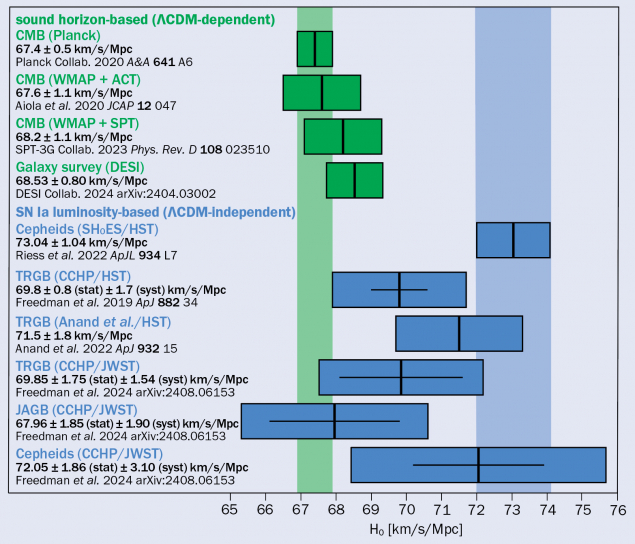
\includegraphics[width=0.9\textwidth]{figures/CCMarApr25_Hubble_tension.jpg}
    \caption[Comparison of local and \ac{CMB}-based measurements of Hubble constant.]{Hubble tension: Comparison of the local and \ac{CMB}-based measurements of $H_0$ over the years~\citep{cern2025}.}
    \label{fig:hubble_tension}
\end{figure}

\subsection{The Hubble Tension and quest for independent measurements}
The Hubble tension, now exceeding $5\sigma$, is one of the most significant unresolved issues in cosmology and has prompted investigations into both systematic errors and possible extensions to the standard cosmological model.
Independent methods are therefore crucial for arbitrating between these measurements. These include:
\begin{itemize}
    \item \textbf{\ac{TRGB}}\\
    The \ac{TRGB} method uses the well-defined luminosity at which low-mass stars ignite helium as a standard candle. This luminosity, shows minimal sensitivity to stellar population effects and dust, making it a robust alternative to Cepheid variables. The Carnegie-Chicago Hubble Program has applied this method to derive an independent calibration of Type Ia supernovae and obtained $H_0$ values closer to those inferred from the CMB~\citep{freedman2024status}. As such, \ac{TRGB} offers a valuable cross-check on the Cepheid-based ladder.
    \item \textbf{\ac{BAO}}\\
    \ac{BAO} are imprints of sound waves in the early Universe, visible as a characteristic scale in the clustering of galaxies. This scale acts as a standard ruler and allows geometric distance measurements across cosmic time. When combined with redshift data and a calibration from the sound horizon measured by the \ac{CMB}, \ac{BAO} can be used to infer $H_0$~\citep{cuceu2019baryon,alam2021completed}. Although \ac{BAO} are not purely local measurements, they offer a powerful, independent cosmological probe that is less susceptible to astrophysical systematics.

    \item \textbf{Gravitational-wave standard sirens}\\
    The use of gravitational-wave events as standard sirens provides a unique opportunity to measure $H_0$ independently.  The use of \ac{GW} sources as \textit{standard sirens}~\citep{schutz1986determining}, provide a direct measurement of the luminosity distance through their waveform. When combined with a redshift, obtained either via electromagnetic counterparts or galaxy catalogs, these events can trace the distance-redshift relation and yield an independent estimate of the Hubble constant.

    Standard sirens can be categoriezed into two broad categories: bright sirens and dark sirens, depending on whether an electromagnetic counterpart is detected. This thesis explores one implementation of this approach, focusing on \textit{dark sirens}: gravitational-wave events without identified electromagnetic counterparts. By statistically associating these events with potential host galaxies in wide-field catalogs, we aim to extract constraints on $H_0$. In particular, we investigate how restricting the galaxy catalog to its brightest subsets can improve the resulting cosmological inference.
\end{itemize}

Together, these emerging methodologies, TRGB, BAO, and standard sirens, form a triangulation of $H_0$ that spans distinct epochs and assumptions. Whether the Hubble tension reflects unknown systematics or fundamentally new physics, its resolution will likely come from the convergence (or divergence) of these independent measurements.

\begin{figure}[h!]
    \centering
    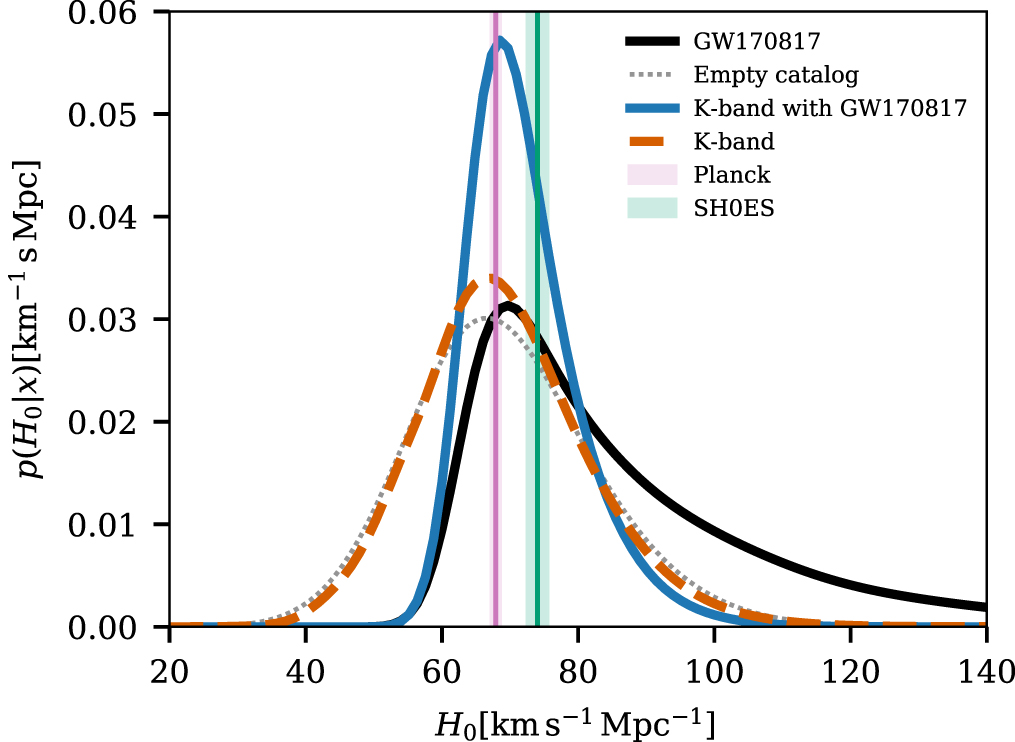
\includegraphics[width=0.8\textwidth]{figures/apjac74bbf9_hr.jpg}
    \caption[Hubble tension and standard sirens]{Hubble constant posterior from \ac{GWTC}-3 released by the \ac{LVK} collaboration, compared to the \ac{CMB} and local measurements. The tension between these measurements is evident, with the \ac{GW} posteriors (blue/orange), with/without the sole bright siren evenet, being consistent with both Planck (pink) and \ac{SH0ES} measurements, owing to the rather wide contraints. Additionally, the empty catalog (gray) and the bright siren (black) results are also plotted~\citep{abbott2023constraints}.}
    \label{fig:hubble_tension_gw}
\end{figure}


\section{\ac{GW} Cosmology}
\ac{GW} observations have introduced a novel, independent method for measuring cosmological distances: the so-called \textit{standard sirens}. First proposed by \citet{schutz1986determining}, standard sirens are the gravitational-wave analogs of \ac{EM} standard candles, such as Type Ia supernovae. Unlike \ac{EM} methods, standard sirens enable a direct, calibration-free determination of the luminosity distance from the observed waveform of a compact binary coalescence.

The amplitude and frequency evolution of the \ac{GW} signal encodes the luminosity distance, which can be inferred under the assumption of general relativity. However, \ac{GW} detectors are not sensitive to the redshift of the source. Therefore, to place a \ac{GW} event on the Hubble diagram and infer the Hubble constant $H_0$, one must independently obtain the redshift.

In the case of bright sirens, events with an \ac{EM} counterpart, such as GW170817~\citep{LIGOScientific:2017adf}, the redshift can be directly measured from the host galaxy spectrum. For the more common class of dark sirens, such as GW170814~\citep{DES:2019ccw}, where no \ac{EM} counterpart is detected, a statistical association is made between the \ac{GW} localization volume and galaxy catalogs. This association yields a redshift probability distribution, which can be combined with the luminosity distance posterior to constrain $H_0$.

The promise of standard sirens lies in their independence from traditional distance ladders and \ac{CMB} modeling. This makes them a crucial tool in addressing the Hubble tension. They are free from many astrophysical systematics affecting \ac{EM} methods, such as dust extinction, metallicity effects, or empirical calibrations. Additionally, because \acp{GW} are less susceptible to environmental interactions, they can probe larger cosmological volumes with fewer intermediate assumptions. As \ac{GW} detectors improve in sensitivity and the number of observed events increases, standard sirens are expected to play a progressively larger role in cosmological inference.

\section{Thesis Objectives}
The primary objective of this thesis is to investigate the impact of using brightness-ranked galaxy catalogs on the precision of $H_0$ measurements from dark sirens. By focusing on the brightest galaxies, we aim to improve the statistical constraints on $H_0$ while minimizing systematic uncertainties associated with galaxy catalog incompleteness.

This work involves $H_0$ inference using the \texttt{gwcosmo} pipeline, which combines \ac{GW} distance posteriors with galaxy redshift priors. We will explore the effects of applying brightness cuts to the galaxy catalog, examining how these cuts influence the resulting $H_0$ posterior distributions. The analysis will be performed on a subset of \ac{GWTC}-3 events, focusing on those with high \acp{SNR} and no known electromagnetic counterparts. The results will be validated through the use of simulated catalogs and mock data challenges, allowing us to assess the robustness of our findings.

In Chapter~\ref{chap:dark-siren-cosmology}, we will provide an overview of the theoretical framework for standard siren cosmology, including the principles of dark sirens. We will also discuss the challenges and limitations associated with this approach, particularly in the context of galaxy catalog incompleteness. Chapter~\ref{chap:data} details the data sources used in our analysis, including the \ac{GW} event catalog and galaxy catalogs. We will describe the selection criteria for the events and the modelling of missing \ac{EM} data. In Chapter~\ref{chap:methodology}, we will detail the methodology used in our analysis, including the construction of brightness-ranked galaxy catalogs and the statistical techniques employed to derive redshift priors. In particular the \texttt{gwcosmo} pipeline will be introduced, which combines the \ac{GW} distance posterior with the galaxy redshift prior to infer $H_0$. In this chapter we also present our results using real data and discusse the impact of brightness cuts on the resulting $H_0$ posterior distributions. In Chapter~\ref{chap:MDC}, we will present the results of our analysis using simulated catalogs and mock data challenges, allowing us to assess the robustness of our findings. Finally, in Chapter~\ref{chap:conclusion}, we will summarize our findings and discuss their implications for future research in cosmology.
